\documentclass{beamer}
\usepackage[english]{babel} %set language; note: after changing this, you need to delete all auxiliary files to recompile
\usepackage[utf8]{inputenc} %define file encoding; latin1 is the other often used option
\usepackage{csquotes} % provides context sensitive quotation facilities
\usepackage{graphicx} %allows for inserting figures
\usepackage{booktabs} % for table formatting without vertical lines
\usepackage{textcomp} % allow for example using the Euro sign with \texteuro
\usepackage{epstopdf} % allow embedding eps-figures
\usepackage{tikz} % allows drawing figures
\usepackage{amsmath,amssymb,amsthm} %advanced math facilities
\usepackage{lmodern} %uses font that support italic and bold at the same time

%add citation management using BibLaTeX
\usepackage[citestyle=authoryear-comp, %define style for citations
    bibstyle=authoryear-comp, %define style for bibliography
    maxbibnames=10, %maximum number of authors displayed in bibliography
    minbibnames=1, %minimum number of authors displayed in bibliography
    maxcitenames=3, %maximum number of authors displayed in citations before using et al.
    minnames=1, %maximum number of authors displayed in citations before using et al.
    datezeros=false, % do not print dates with leading zeros
    date=long, %use long formats for dates
    isbn=false,% show no ISBNs in bibliography (applies only if not a mandatory field)
    url=false,% show no urls in bibliography (applies only if not a mandatory field)
    doi=false, % show no dois in bibliography (applies only if not a mandatory field)
    eprint=false, %show no eprint-field in bibliography (applies only if not a mandatory field)
    backend=biber %use biber as the backend; backend=bibtex is less powerful, but easier to install
    ]{biblatex}
\addbibresource{../mybibfile.bib} %define bib-file located one folder higher


\usefonttheme[onlymath]{serif} %set math font to serif ones

\definecolor{beamerblue}{rgb}{0.2,0.2,0.7} %define beamerblue color for later use

%%% defines highlight command to set text blue
\newcommand{\highlight}[1]{{\color{blue}{#1}}}


%%%%%%% commands defining backup slides so that frame numbering is correct

\newcommand{\backupbegin}{
   \newcounter{framenumberappendix}
   \setcounter{framenumberappendix}{\value{framenumber}}
}
\newcommand{\backupend}{
   \addtocounter{framenumberappendix}{-\value{framenumber}}
   \addtocounter{framenumber}{\value{framenumberappendix}}
}

%%%% end of defining backup slides

%Specify figure caption, see also http://tex.stackexchange.com/questions/155738/caption-package-not-working-with-beamer
\setbeamertemplate{caption}{\insertcaption} %redefines caption to remove label "Figure".
%\setbeamerfont{caption}{size=\scriptsize,shape=\itshape,series=\bfseries} %sets figure  caption bold and italic and makes it smaller


\usetheme{Boadilla}

%set options of hyperref package
\hypersetup{
    bookmarksnumbered=true, %put section numbers in bookmarks
    naturalnames=true, %use LATEX-computed names for links
    citebordercolor={1 1 1}, %color of border around cites, here: white, i.e. invisible
    linkbordercolor={1 1 1}, %color of border around links, here: white, i.e. invisible
    colorlinks=true, %color links
    anchorcolor=black, %set color of anchors
    linkcolor=beamerblue, %set link color to beamer blue
    citecolor=blue, %set cite color to beamer blue
    pdfpagemode=UseThumbs, %set default mode of PDF display
    breaklinks=true, %break long links
    pdfstartpage=1 %start at first page
    }


% --------------------
% Overall information
% --------------------
\title{Your title goes here}
\date{\today}
\author{Johannes Pfeifer}
\institute{University of Cologne}


\begin{document}

\begin{frame}
  \titlepage
\end{frame}


\begin{frame}
    \tableofcontents
\end{frame}

\section{Introduction}
\begin{frame}{Latex Beamer: Read the manual}
    \begin{itemize}
        \item All commands can be looked up in the beamer manual at
            \url{http://www.tex.ac.uk/tex-archive/macros/latex/contrib/beamer/doc/beameruserguide.pdf}
        \item Most important is Part III of the manual that explains how to change the layout
        \item For example, try replacing the theme \textit{Boadilla} with \textit{Warsaw} in the preamble of this file
    \end{itemize}
\end{frame}


\subsection{This is subsection 1}
\begin{frame}{Frame Title: A slide with a figure above a list}
    \begin{figure}
        \includegraphics[scale=.3]{why_has_the_recovery_been_so_slow_all_respondents_0}
        \caption{Source: The Economist, October 5th}
    \end{figure}
    \begin{itemize}
        \item Description goes here
    \end{itemize}
\end{frame}

\section{The Model}
\subsection{This is subsection 1}

\begin{frame}{Figure and list side by side}
    \begin{figure}[htbp!]
        \begin{minipage}{0.55\linewidth}
            \includegraphics[height=5cm,width=6cm]{smoothedvariances}
            \caption{Source:  \textcite{BornPfeifer2014JME}}
        \end{minipage}
        \begin{minipage}{0.4\linewidth}
            \begin{itemize}
            \item The \texttt{height} and \texttt{width} options allow stretching the figure
            \item Insert item
            \end{itemize}
        \end{minipage}
    \end{figure}
\end{frame}


\begin{frame}{Link to Backup Slide}\label{modelstructure} %label is required for jump button back
        \begin{itemize}
            \item Some text
            \item Beamer also allows math:
            \begin{equation}
                e^{i\pi}-1=0 \quad ,
            \end{equation}
            where $i=\sqrt{-1}$
        \end{itemize}
\hyperlink{model_appendix}{\beamergotobutton{Model Details}} % defines hyperlink associated with certain button type and name
\end{frame}



\subsection{This is subsection 2}
\begin{frame}{Slide with list that is revealed in steps}
    \begin{itemize}[<+->]
        \item First item
        \item Second item
    \end{itemize}
\end{frame}


\begin{frame}{Slide with enumeration and highlighting}
    Three items in a numbered list
    \begin{enumerate}
        \item List item one
        \item \highlight{List item two}
        \item \alert{List item three}
    \end{enumerate}
\end{frame}

\begin{frame}{Tables also work in normal \LaTeX}
    \begin{table}
    \caption{Title of the table} % the title is often not needed due to the frametitle
    \label{tab:Table1}
    \centering
         \begin{tabular}{lcr}
               A & small  & table\\
            \toprule
               left aligned & centered & right aligned \\
               & two lines separated by a line  & \\
            \cmidrule{2-3}
               \multicolumn{2}{c}{Text over two columns} & third column \\
            \bottomrule\\
        \end{tabular}\\
    \footnotesize{\emph{Notes:} Add the description here}
    \end{table}
\end{frame}



\begin{frame}{Self-drawn pictures using Tikz}
\begin{figure}
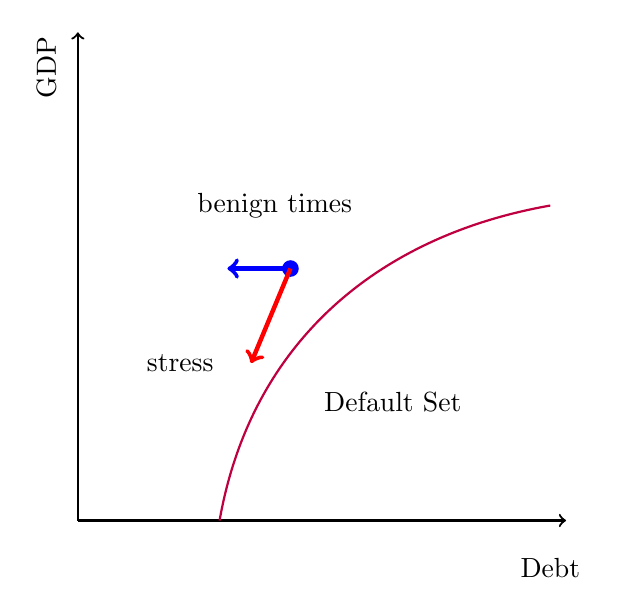
\begin{tikzpicture}[domain=0:5,range=1:5,scale=1,thick]
\usetikzlibrary{calc} %all
%Draw axes, and dotted equilibrium lines.
\draw [->] (0,0) -- (6.2,0);
\node at (6,-0.6) {Debt};
\draw [->] (0,0) -- (0,6.2);
\node[rotate=90] at (-0.4,5.75) {GDP};
\coordinate (A) at (2.7,3.2);
\fill[blue] (A) circle (3pt);

\draw[thick,color=purple] (1.8,0) to [out=80,in=190] (6,4);
\node at (4,1.5) {Default Set};

%the following part only appears on the second and third slide
\visible<2-3>{
\node at (2.5,4) {benign times};
\draw[->,ultra thick,color=blue] (A) -- (1.9,3.2);
}
%the following part only appears on the third slide
\visible<3-3>{
\node at (1.3,2) {stress};
\draw[->,ultra thick,color=red] (A) -- (2.2,2);
}

\end{tikzpicture}
\caption{Source: \textcite{BMP2015}}
\end{figure}

\end{frame}
\section{Conclusion and Summary}

\begin{frame}{Summary with nested lists}
    \begin{itemize}
        \item Item 1
        \item Item 2
        \begin{itemize}
            \item Subitem 1
            \item
        \end{itemize}
    \end{itemize}
\end{frame}


\appendix

\backupbegin %defines begin of backup slides so the numbering stops

\begin{frame}{First Backup Slide}\label{model_appendix}
    \begin{itemize}
        \item Item 1
        \item Item 2
        \begin{itemize}
            \item Subitem 1
            \item
        \end{itemize}
    \end{itemize}

    \hyperlink{modelstructure}
    {\beamerreturnbutton{Model Details}}
\end{frame}

%add the Bibliography
\begin{frame}[allowframebreaks]{Bibliography}
\printbibliography
\end{frame}

\backupend % end of backup slides

\end{document}
